\documentclass{beamer}
\usepackage[utf8]{inputenc}

\usetheme{Madrid}
\usecolortheme{default}
\usepackage{amsmath,amssymb,amsfonts,amsthm}
\usepackage{txfonts}
\usepackage{tkz-euclide}
\usepackage{listings}
\usepackage{adjustbox}
\usepackage{array}
\usepackage{tabularx}
\usepackage{gvv}
\usepackage{lmodern}
\usepackage{circuitikz}
\usepackage{tikz}
\usepackage{graphicx}

\setbeamertemplate{page number in head/foot}[totalframenumber]

\usepackage{tcolorbox}
\tcbuselibrary{minted,breakable,xparse,skins}



\definecolor{bg}{gray}{0.95}
\DeclareTCBListing{mintedbox}{O{}m!O{}}{%
  breakable=true,
  listing engine=minted,
  listing only,
  minted language=#2,
  minted style=default,
  minted options={%
    linenos,
    gobble=0,
    breaklines=true,
    breakafter=,,
    fontsize=\small,
    numbersep=8pt,
    #1},
  boxsep=0pt,
  left skip=0pt,
  right skip=0pt,
  left=25pt,
  right=0pt,
  top=3pt,
  bottom=3pt,
  arc=5pt,
  leftrule=0pt,
  rightrule=0pt,
  bottomrule=2pt,
  toprule=2pt,
  colback=bg,
  colframe=orange!70,
  enhanced,
  overlay={%
    \begin{tcbclipinterior}
    \fill[orange!20!white] (frame.south west) rectangle ([xshift=20pt]frame.north west);
    \end{tcbclipinterior}},
  #3,
}
\lstset{
    language=C,
    basicstyle=\ttfamily\small,
    keywordstyle=\color{blue},
    stringstyle=\color{orange},
    commentstyle=\color{green!60!black},
    numbers=left,
    numberstyle=\tiny\color{gray},
    breaklines=true,
    showstringspaces=false,
}
\title{2.10.74}
\date{9th September, 2025}
\author{Puni Aditya - EE25BTECH11046}

\begin{document}

\frame{\titlepage}
\begin{frame}{Question}
If $\vec{X} \cdot \vec{A} = 0$, $\vec{X} \cdot \vec{B} = 0$, and $\vec{X} \cdot \vec{C} = 0$ for some non-zero vector $\vec{X}$, then $\sbrak{\vec{A}\ \vec{B}\ \vec{C}} = 0$.
\end{frame}

\begin{frame}{Theoretical Solution}
\begin{align}
    \vec{X} \cdot \vec{A} = 0 \label{eq:1} \\
    \vec{X} \cdot \vec{B} = 0 \label{eq:2} \\
    \vec{X} \cdot \vec{C} = 0 \label{eq:3}
\end{align}

From \eqref{eq:1}, \eqref{eq:2} and \eqref{eq:3},
\begin{align}
    \vec{A}^\top \vec{X} = \vec{B}^\top \vec{X} = \vec{C}^\top \vec{X} = 0
\end{align}
\end{frame}

\begin{frame}{Theoretical Solution}
This forms the set of equations
\begin{align}
    \myvec{\vec{A}^\top \\ \vec{B}^\top \\ \vec{C}^\top} \vec{X} &= \myvec{0 \\ 0 \\ 0} \\
    \myvec{\vec{A} & \vec{B} & \vec{C}}^\top\vec{X} &= \vec{0}
\end{align}
For a homogeneous set of equations to have non-trivial solution $\vec{X}$, the coefficient matrix is singular.
\begin{align*}
    \implies \myvec{\vec{A} & \vec{B} & \vec{C}}^\top\text{ is singular.}
\end{align*}

\begin{align*}
    \implies \myvec{\vec{A} & \vec{B} & \vec{C}}\text{ is singular since }\myvec{\vec{A} & \vec{B} & \vec{C}}\text{ is square.}
\end{align*}
\begin{align*}
    \therefore \sbrak{\vec{A}\ \vec{B}\ \vec{C}} = 0
\end{align*}

Hence, the given statement is true. \\

\end{frame}

\begin{frame}{Example}
Let
\begin{align*}
    \vec{X}=\myvec{1 \\ 1 \\ 1}, \vec{A}=\myvec{1 \\ -1 \\ 0}, \vec{B}=\myvec{1 \\ 0 \\ -1}, \vec{C}=\myvec{0 \\ 1 \\ -1}
\end{align*}
\begin{align}
    \vec{A}^\top \vec{X} = \vec{B}^\top \vec{X} = \vec{C}^\top \vec{X} = 0\text{ for this example.}
\end{align}
\begin{align}
    \sbrak{\vec{A}\ \vec{B}\ \vec{C}} = \myvec{1 & -1 & 0}\brak{\myvec{1 \\ 0 \\ -1}\times\myvec{0 \\ 1 \\ -1}}
\end{align}
\begin{align}
    \sbrak{\vec{A}\ \vec{B}\ \vec{C}} &= \myvec{1 & -1 & 0} \myvec{1 \\ 1 \\ 1} \\
    \sbrak{\vec{A}\ \vec{B}\ \vec{C}} &= 0
\end{align}
\end{frame}

\begin{frame}{Plot}
    \begin{figure}
        \centering
        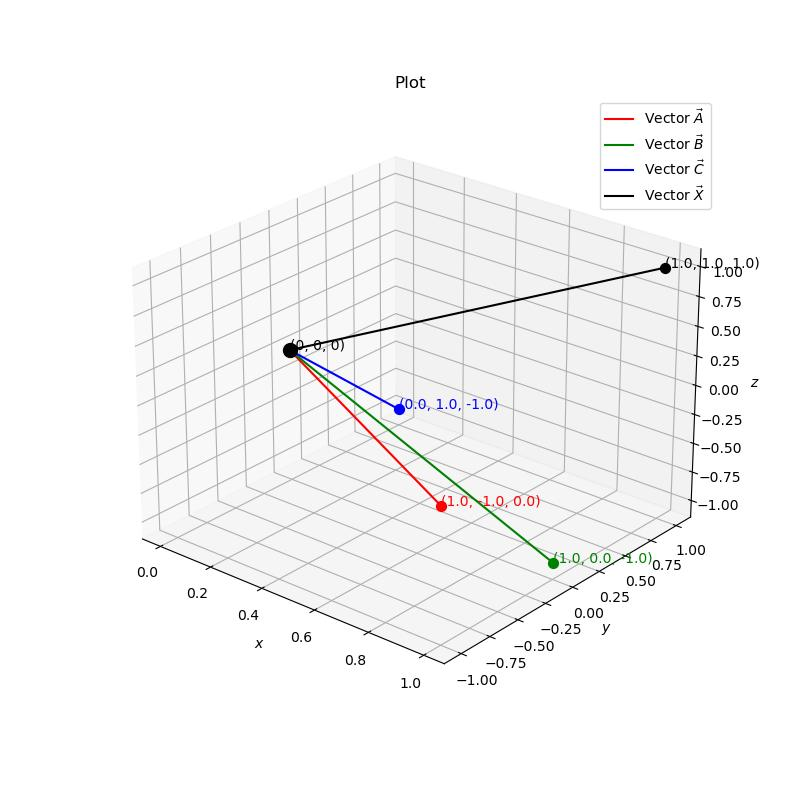
\includegraphics[width=0.5\columnwidth]{../figs/plot_c.jpg}
        \caption{Example}
        \label{fig:fig}
    \end{figure}
\end{frame}

\end{document}
